
\documentclass{mcmthesis}
\mcmsetup{CTeX = true,   % 使用 CTeX 套装时,设置为 true
        tcn = 0000, problem = A,
        sheet = true, titleinsheet = true, keywordsinsheet = true,
        titlepage = true, abstract = true}
\usepackage{newtxtext}%\usepackage{palatino}
\usepackage{lipsum}
\usepackage{subfigure}
\title{The \LaTeX{} Template for MCM Version \MCMversion}
\author{\small \href{https://www.latexstudio.net/}
  {\includegraphics[width=7cm]{mcmthesis-logo}}}
\date{\today}
\begin{document}
\begin{abstract}
% 摘要


\begin{keywords}
% 关键词
keyword1; keyword2


\end{keywords}
\end{abstract}
\maketitle
%% Generate the Table of Contents, if it's needed.
%% \tableofcontents
%% \newpage
%%
%% Generate the Memorandum, if it's needed.
%% \memoto{\LaTeX{}studio}
%% \memofrom{Liam Huang}
%% \memosubject{Happy \TeX{}ing!}
%% \memodate{\today}
%% \logo{\LARGE I'm pretending to be a LOGO!}
%% \begin{memo}[Memorandum]
%%   \lipsum[1-3]
%% \end{memo}
%%

\newpage
\thispagestyle{empty}
\tableofcontents
\newpage



\section{Introduction}
\subsection{Background}
随着个人资产的累计,越来越多的人进入投资市场,为了在使现有资产保值或更有价值。
但我们都知道,投资类产品常有很强的波动性,which means 它很难预测。
在众多投资产品中,黄金和比特币最受人关注。
特别是比特币,自出现以来交易规模迅速扩张,但巨大的价格波动使其安全性和稳定性受到质疑。
那么,在黄金和比特币投资热潮下,对普通交易者大幅度得利的投资组合很难实现。
这是很重要的,根据每天和前几天更新的交易数据,来预测未来波动性资产的发展趋势。
因此,交易者提出 to develop a model that uses only the past stream of daily prices 
to date to determine each day if the trader should buy, hold, or sell their assets in their portfolio.


\subsection{Problem Statement}


\subsection{Problem Analysis}
为了更好的帮助交易者做出每日投资决策,我们







\section{Assumption}



\section{Data Processing}
\subsection{Data Screening}

\subsection{Data Visualization}

\subsection{Mining Time Series}
\subsubsection{Stability Test}

\subsubsection{White Noise Test}



\section{PartⅠ:Model Development }
\subsection{Time Series Model ARIMA - Data Forecasting }

\subsubsection{Train the Model With All the Data}

\subsubsection{Model Validating}

\subsubsection{Model Prediction and Visualization}

\subsubsection{Batch prediction of data }   %去未来七天


\subsection{Investment Decision Model - Dynamic Programming }
%流程图
\iffalse
\begin{figure}[!hb]
    \centering  %图片居中显示        %路径不能有中文
    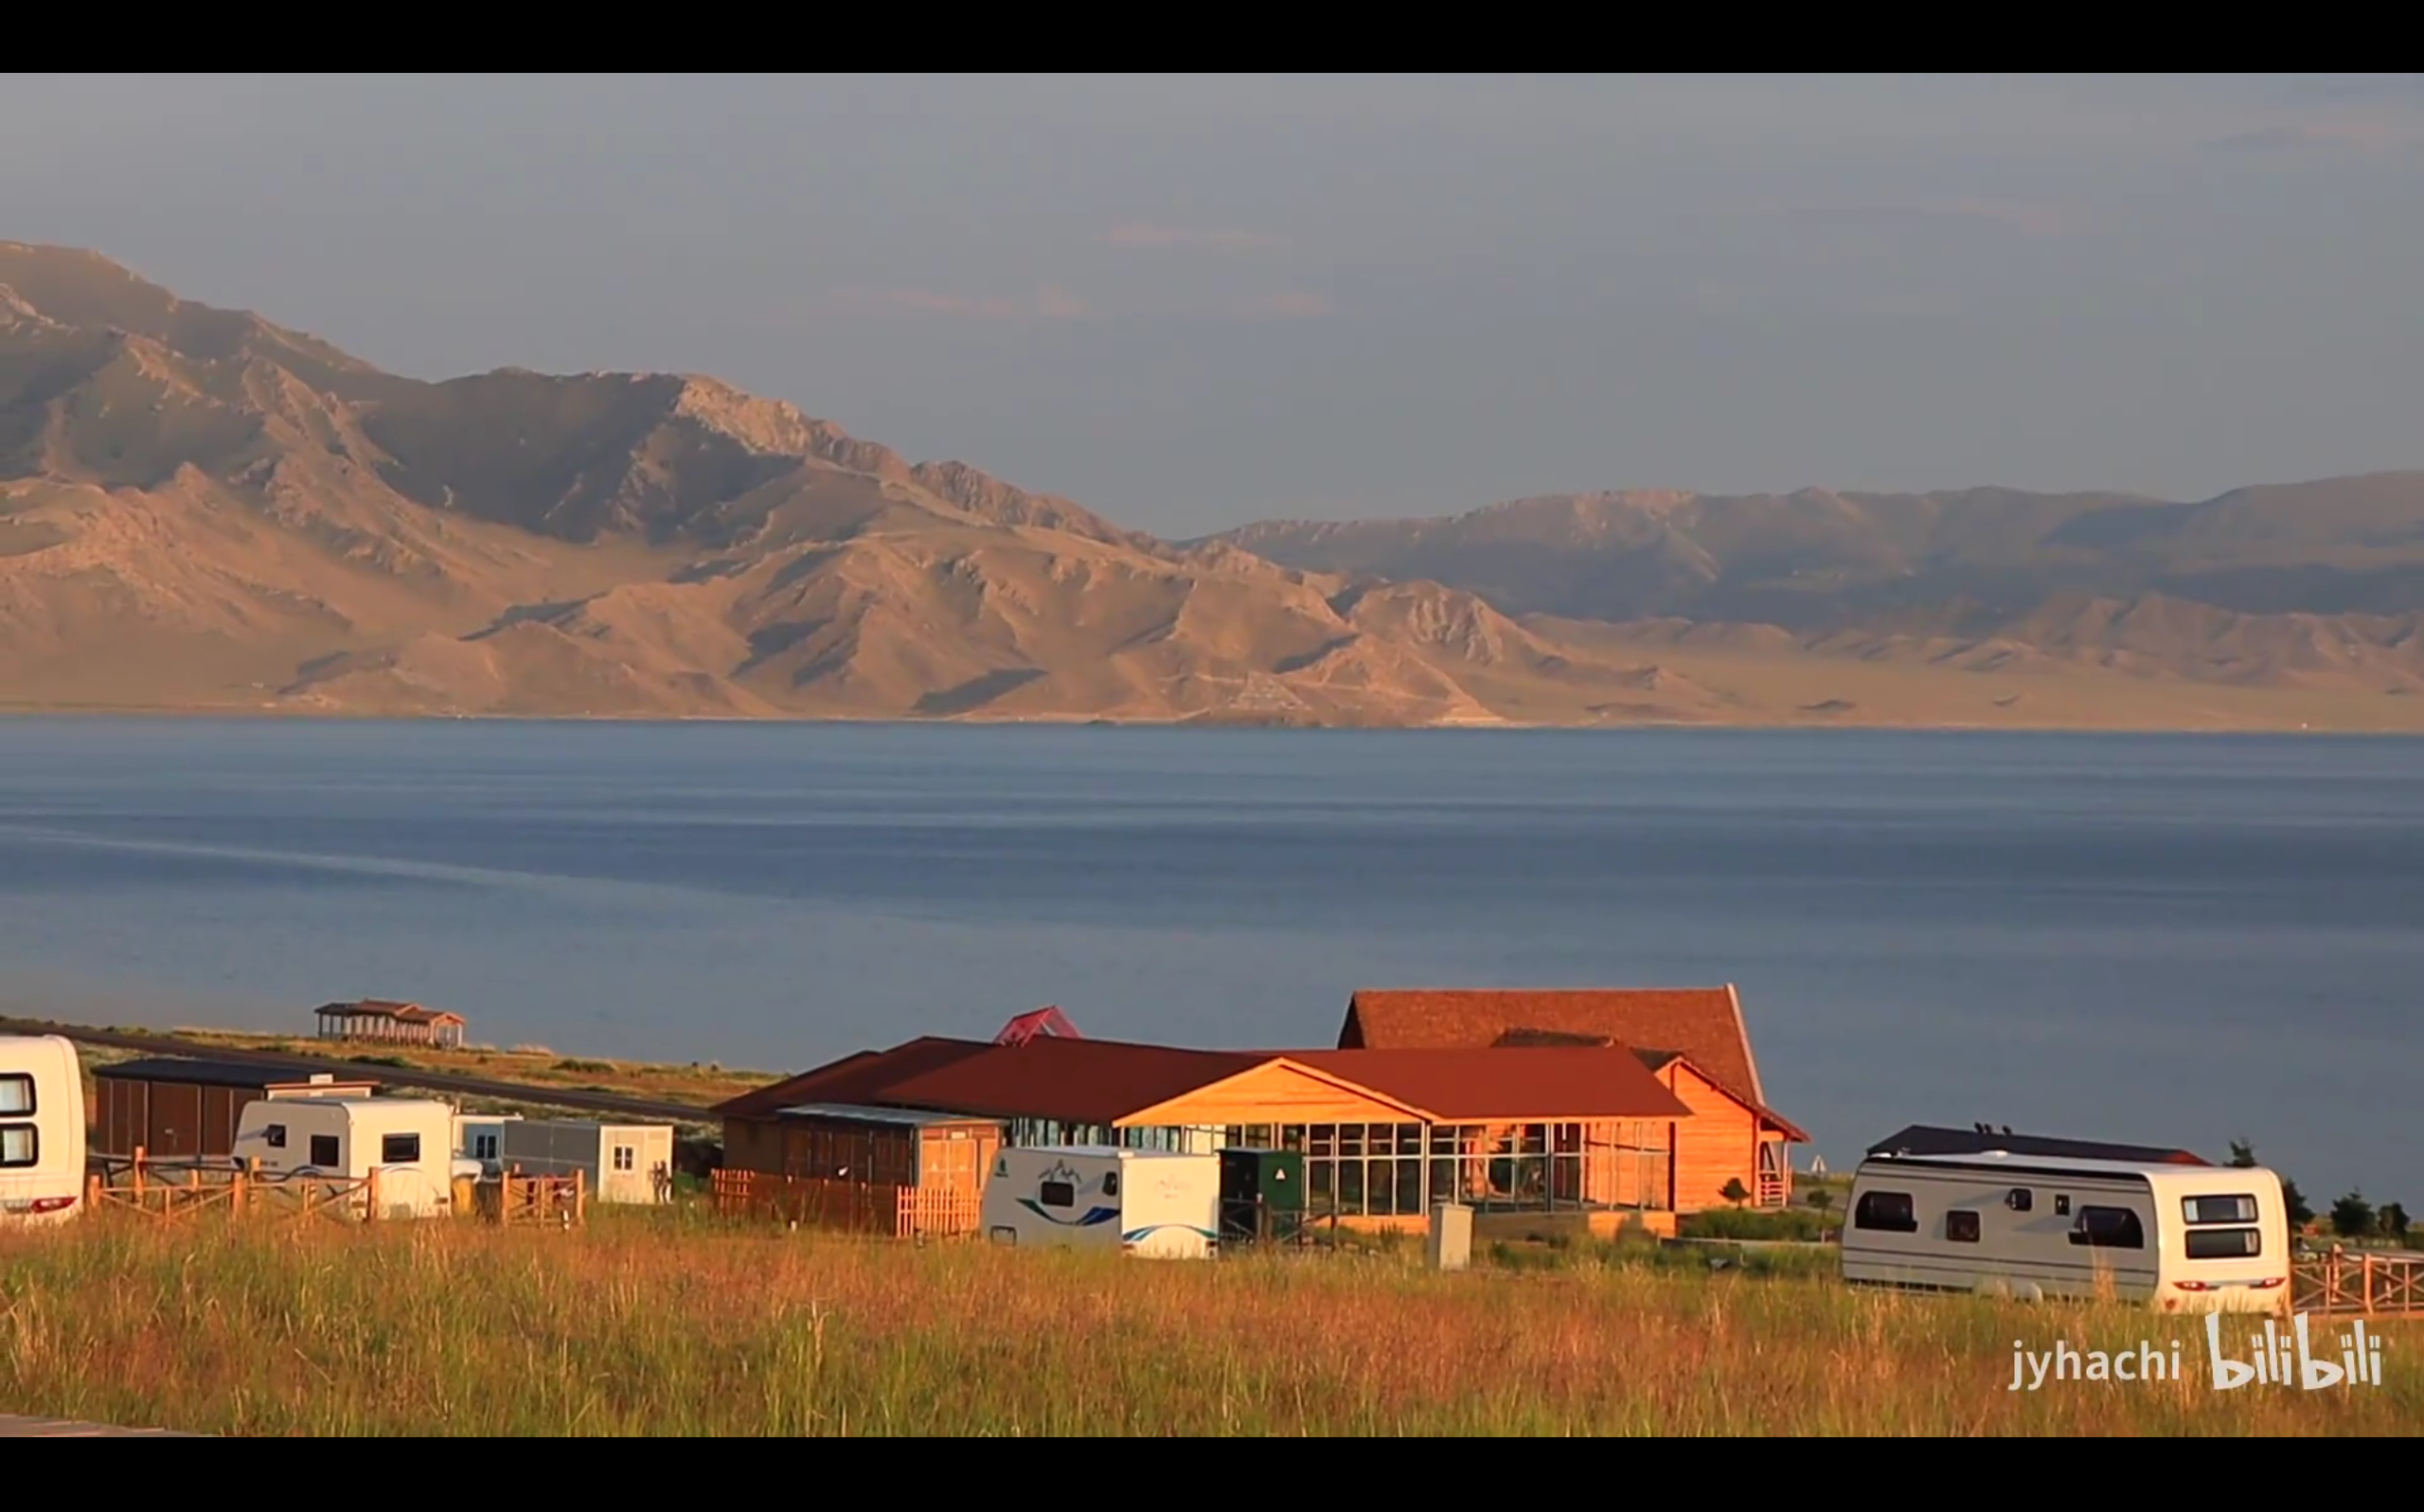
\includegraphics[width=3cm]{jinyue.png}
    \caption{这是美丽喀纳斯} \label{kanasi}
 \end{figure}
\fi

\subsubsection{Buy and Sell Standard Setting}

\subsubsection{Portfolio Optimal Ratio Identification}

\subsubsection{Positioning Standard Identification}

\subsubsection{Daily Portfolio Determinations}






\section{PartⅡ:Strategy Evaluation}
\subsection{Set Perturbation Terms }%to determine optimal parameters }

\subsection{Comparison Illustrates the Best Strategy}




\section{PartⅢ:Sensitivity Analysis}
\subsection{Assuming Changes In Commission}

\subsection{Visualization Results}%Analysis ensitivity}





\section{Evaluate of the Model}
\subsection{Strengths and weaknesses}

\subsection{Sensitivity Analysis}




\section{Conclusions}


\section{A Memo}








\begin{thebibliography}{99}
\bibitem{1} D.~E. KNUTH   The \TeX{}book  the American
Mathematical Society and Addison-Wesley
Publishing Company , 1984-1986.
\bibitem{2}Lamport, Leslie,  \LaTeX{}: `` A Document Preparation System '',
Addison-Wesley Publishing Company, 1986.
\bibitem{3}\url{https://www.latexstudio.net/}
\end{thebibliography}

\begin{appendices}

\section{First appendix}

In addition, your report must include a letter to the Chief Financial Officer (CFO) of the Goodgrant Foundation, Mr. Alpha Chiang, that describes the optimal investment strategy, your modeling approach and major results, and a brief discussion of your proposed concept of a return-on-investment (ROI). This letter should be no more than two pages in length.







\begin{letter}{Dear, Mr. Alpha Chiang}

\vspace{\parskip}

Sincerely yours,

Your friends

\end{letter}
Here are simulation programmes we used in our model as follow.\\

\textbf{\textcolor[rgb]{0.98,0.00,0.00}{Input matlab source:}}
\lstinputlisting[language=Matlab]{./code/mcmthesis-matlab1.m}

\section{Second appendix}

some more text \textcolor[rgb]{0.98,0.00,0.00}{\textbf{Input C++ source:}}
\lstinputlisting[language=C++]{./code/mcmthesis-sudoku.cpp}

\end{appendices}
\end{document}
%% 
%% This work consists of these files mcmthesis.dtx,
%%                                   figures/ and
%%                                   code/,
%% and the derived files             mcmthesis.cls,
%%                                   mcmthesis-demo.tex,
%%                                   README,
%%                                   LICENSE,
%%                                   mcmthesis.pdf and
%%                                   mcmthesis-demo.pdf.
%%
%% End of file `mcmthesis-demo.tex'.